% This LaTeX was auto-generated from MATLAB code.
% To make changes, update the MATLAB code and export to LaTeX again.

\documentclass{article}

\usepackage[utf8]{inputenc}
\usepackage[T1]{fontenc}
\usepackage{lmodern}
\usepackage{graphicx}
\usepackage{color}
\usepackage{hyperref}
\usepackage{amsmath}
\usepackage{amsfonts}
\usepackage{epstopdf}
\usepackage[table]{xcolor}
\usepackage{matlab}

\sloppy
\epstopdfsetup{outdir=./}
\graphicspath{ {./HW10_code_images/} }

\matlabhastoc

\matlabmultipletitles

\begin{document}

\maketitle
\thispagestyle{empty}
\pagebreak
\matlabtableofcontents{Table of Contents}

\begin{par}
\begin{flushleft}
In this homework assignment, LeNet-5 neural network is used to classify MNIST handwritten digits into 10 classes.
\end{flushleft}
\end{par}

\begin{matlabcode}
clc; clear; close all;
load('HW10_code_workspace.mat');
\end{matlabcode}
\pagebreak

\label{T_AF22880B}
\matlabtitle{0. MNIST Dataset}

\label{H_FBA02D0E}
\matlabheading{0.1 Downloading MNIST Dataset and Import into \textit{Matlab}}

\begin{par}
\begin{flushleft}
The code snippet below will download MNIST dataset from web and extract the downloaded file into Matlab matrices as test and train images and labels.
\end{flushleft}
\end{par}

\begin{matlabcode}
mnist_train_image = 'train-images-idx3-ubyte';
mnist_train_label = 'train-labels-idx1-ubyte';
mnist_test_image  = 't10k-images-idx3-ubyte';
mnist_test_label  = 't10k-labels-idx1-ubyte';
train_set_number  = 60000;
test_set_number   = 10000;

downloadMNIST(mnist_train_image, mnist_train_label, mnist_test_image, mnist_test_label);
\end{matlabcode}
\begin{matlaboutput}
MNIST dataset already downloaded.
\end{matlaboutput}


\begin{matlabcode}
[train_images, train_labels] = readMNIST(mnist_train_image, mnist_train_label, train_set_number);
[test_images,   test_labels] = readMNIST(mnist_test_image, mnist_test_label, test_set_number);

clear mnist_train_image mnist_train_label mnist_test_image mnist_test_label train_set_number test_set_number
\end{matlabcode}


\label{H_3C76610B}
\matlabheading{0.2 Plotting a Sample of MNIST Dataset}

\begin{par}
\begin{flushleft}
A set of 100 randomly chosen samples of the training dataset is plotted here.
\end{flushleft}
\end{par}

\begin{matlabcode}
random_indices = randi(60000, [1 100]);
montage(train_images(:, :, random_indices), 'BorderSize', [2 2], 'BackgroundColor', 'white');
\end{matlabcode}
\begin{center}
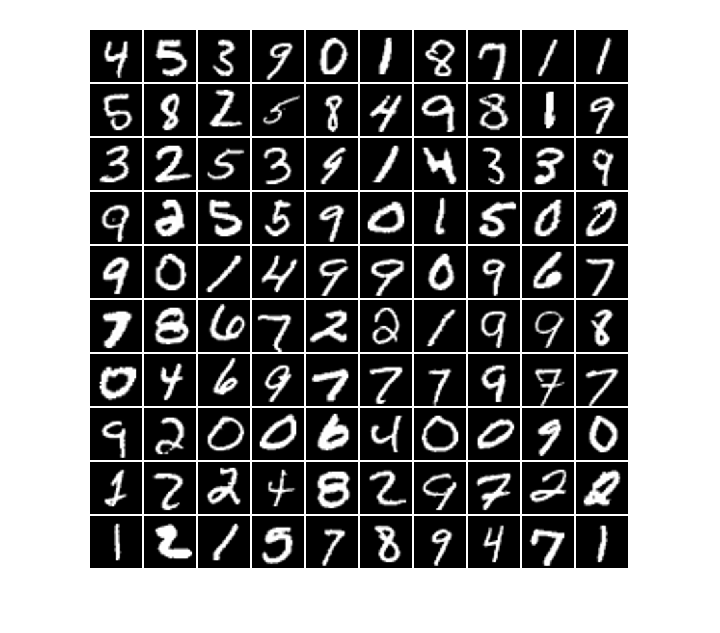
\includegraphics[width=\maxwidth{72.25288509784245em}]{figure_0.png}
\end{center}


\label{H_CF10BD53}
\matlabheading{0.3 Splitting MNIST into Folders by Their Labels}

\begin{par}
\begin{flushleft}
After downloading the dataset, we need to put every single image in a folder which has the name equal to the image's label. By doing so, it will make it easier for us to take advantage of Matlab built-in functions to load the dataset into matlab workspace.
\end{flushleft}
\end{par}

\begin{matlabcode}
if ~exist('mnistTrain','dir')
    disp('Saving the Images in folders. This might take some time...');
    saveMNISTasFolderOfImages(pwd, train_images, train_labels, test_images, test_labels);
else
    disp('MNIST dataset already foldered!')
end
\end{matlabcode}
\begin{matlaboutput}
MNIST dataset already foldered!
\end{matlaboutput}


\label{H_04AC7514}
\matlabheading{0.4 Loading Training Images into \textit{Matlab}}

\begin{par}
\begin{flushleft}
Here we have loaded the training images as \textit{\textbf{imageDataStore}} type in Matlab because large datasets are handled more easily with this specific type.
\end{flushleft}
\end{par}

\begin{matlabcode}
categories = {'0','1','2','3','4','5','6','7','8','9'};

rootFolder = 'mnistTrain';
imds = imageDatastore(fullfile(rootFolder, categories), ...
    'LabelSource', 'foldernames');
clear rootFolder

disp(countEachLabel(imds));
\end{matlabcode}
\begin{matlaboutput}
    Label    Count
    _____    _____

      0      5923 
      1      6742 
      2      5958 
      3      6131 
      4      5842 
      5      5421 
      6      5918 
      7      6265 
      8      5851 
      9      5949 
\end{matlaboutput}


\label{H_0C5B18D4}
\matlabheading{0.5 Plot One Random Sample of Each Class}

\begin{par}
\begin{flushleft}
We plot one sample of every class in the training dataset with a color-bar which represents their pixel range values.
\end{flushleft}
\end{par}

\begin{matlabcode}
rand_nums = randi(size(imds.Files, 1)/10) + [0:6000:54000];

figure('Position', [100, 100, 1000, 500]);
for i = 1:10
    subplottight(2, 5, i);
    imshow(imread(imds.Files{rand_nums(i)}), 'border', 'tight');
    title(char(imds.Labels(rand_nums(i))));
    colorbar('westoutside');
    hold on;
end

hold off
\end{matlabcode}
\begin{center}
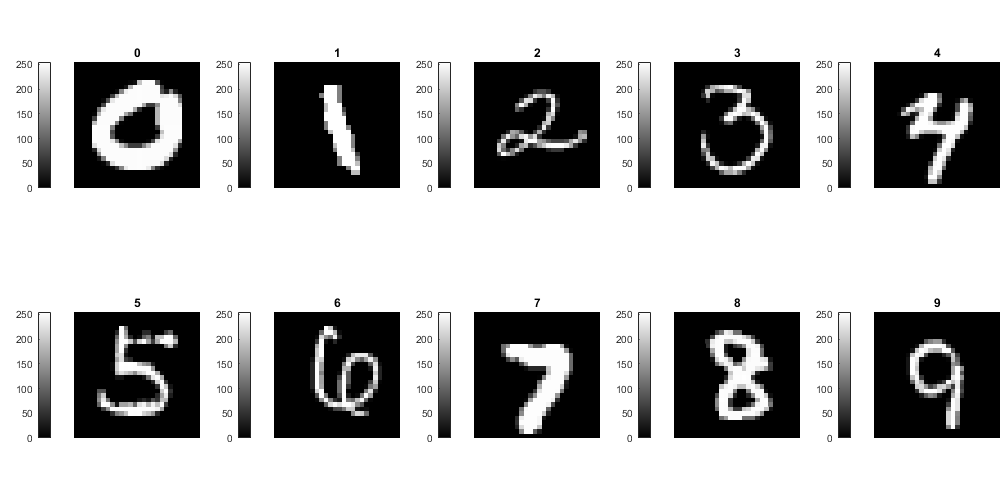
\includegraphics[width=\maxwidth{80.28098344204717em}]{figure_1.png}
\end{center}
\pagebreak

\label{T_802C2325}
\matlabtitle{1. LeNet-5 Training}

\begin{par}
\begin{flushleft}
In this section we will define and train a neural network according to \href{http://vision.stanford.edu/cs598_spring07/papers/Lecun98.pdf}{[lecun et al., 1998]} paper.
\end{flushleft}
\end{par}

\label{H_C64558E1}
\matlabheading{1.1 Defining LeNet-5 Architecture}

\begin{par}
\begin{flushleft}
Input size in lecun's paper was 32x32 images however downloaded MNIST images are of size 28x28. Therefore we have used 'same' padding for the first convolutional layer (C1). By doing so, the dimension fo the rest of the neural network will be the same to the original paper.
\end{flushleft}
\end{par}

\begin{matlabcode}
LeNet_5 = [
    imageInputLayer([28 28], 'Name', 'data')
    
    convolution2dLayer([5 5], 6, 'Name', 'C1', 'Stride', [1 1], 'Padding', 'same')
    tanhLayer('Name','tanh1')
    
    averagePooling2dLayer([2 2], 'Name', 'S2', 'Stride', [2 2])
    
    convolution2dLayer([5 5], 16, 'Name', 'C3', 'Stride', [1 1])
    tanhLayer('Name','tanh3')
    
    averagePooling2dLayer([2 2], 'Name', 'S4', 'Stride', [2 2])
    
    convolution2dLayer([5 5], 120, 'Name', 'C5', 'Stride', [1 1])
    tanhLayer('Name','tanh5')

    fullyConnectedLayer(84, 'Name', 'F6')
    tanhLayer('Name','tanh6')
    
    fullyConnectedLayer(10, 'Name', 'output')
    softmaxLayer('Name','softmax')
    
    classificationLayer('Name','classification')
    ];

disp(LeNet_5);
\end{matlabcode}
\begin{matlaboutput}
  14x1 Layer array with layers:

     1   'data'             Image Input             28x28x1 images with 'zerocenter' normalization
     2   'C1'               Convolution             6 5x5 convolutions with stride [1  1] and padding 'same'
     3   'tanh1'            Tanh                    Hyperbolic tangent
     4   'S2'               Average Pooling         2x2 average pooling with stride [2  2] and padding [0  0  0  0]
     5   'C3'               Convolution             16 5x5 convolutions with stride [1  1] and padding [0  0  0  0]
     6   'tanh3'            Tanh                    Hyperbolic tangent
     7   'S4'               Average Pooling         2x2 average pooling with stride [2  2] and padding [0  0  0  0]
     8   'C5'               Convolution             120 5x5 convolutions with stride [1  1] and padding [0  0  0  0]
     9   'tanh5'            Tanh                    Hyperbolic tangent
    10   'F6'               Fully Connected         84 fully connected layer
    11   'tanh6'            Tanh                    Hyperbolic tangent
    12   'output'           Fully Connected         10 fully connected layer
    13   'softmax'          Softmax                 softmax
    14   'classification'   Classification Output   crossentropyex
\end{matlaboutput}


\begin{par}
\begin{flushleft}
In the figure below, we can see the whole network at a glance:
\end{flushleft}
\end{par}

\begin{matlabcode}
analyzeNetwork(LeNet_5);
plot(layerGraph(LeNet_5));
\end{matlabcode}
\begin{center}
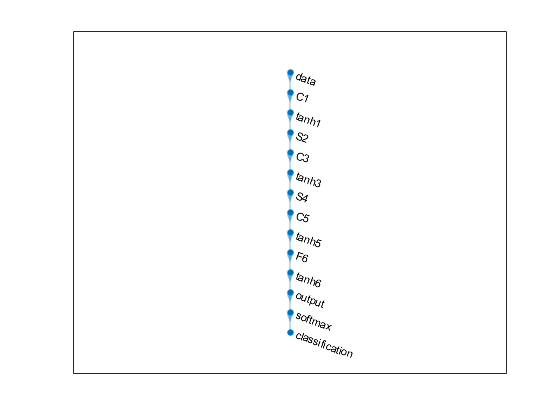
\includegraphics[width=\maxwidth{56.196688409433015em}]{figure_2.png}
\end{center}


\label{H_51FEB5DB}
\matlabheading{1.2 Split Training Data into \textit{train} and \textit{validation }Subsets}

\begin{par}
\begin{flushleft}
15 percent of the 60,000 training images are assigned to the validation set and the rest are kept for the neural network training.
\end{flushleft}
\end{par}

\begin{matlabcode}
[imdsTrain, imdsValidation] = splitEachLabel(imds,0.85,'randomized');
disp(countEachLabel(imdsTrain));
\end{matlabcode}
\begin{matlaboutput}
    Label    Count
    _____    _____

      0      5035 
      1      5731 
      2      5064 
      3      5211 
      4      4966 
      5      4608 
      6      5030 
      7      5325 
      8      4973 
      9      5057 
\end{matlaboutput}
\begin{matlabcode}
disp(countEachLabel(imdsValidation));
\end{matlabcode}
\begin{matlaboutput}
    Label    Count
    _____    _____

      0       888 
      1      1011 
      2       894 
      3       920 
      4       876 
      5       813 
      6       888 
      7       940 
      8       878 
      9       892 
\end{matlaboutput}


\label{H_93FF252C}
\matlabheading{1.3 Defining Options for Training}

\begin{par}
\begin{flushleft}
We have used 15 epoches with mini-batch size of 512 to train the network.
\end{flushleft}
\end{par}

\begin{matlabcode}
opts = trainingOptions('adam', ...
    'ExecutionEnvironment','auto', ...
    'MaxEpochs', 15, ...
    'MiniBatchSize', 512, ...
    'Shuffle', 'every-epoch', ...
    'Plots', 'training-progress', ...
    'Verbose', true, ...
    'ValidationData', imdsValidation);
\end{matlabcode}


\label{H_19DBC5FC}
\matlabheading{1.4 Learning Curves and Training Process}

\begin{par}
\begin{flushleft}
We trained the network on single GPU system. The results are printed in a table every 50 iterations. Besides, the learning curves are plotted after the table. Finally the network reached 98.44\% on training and 98.91\% on validation subset. The training process took about 5 minutes long.
\end{flushleft}
\end{par}

\begin{matlabcode}
trained_LeNet_5 = trainNetwork(imdsTrain, LeNet_5, opts);
\end{matlabcode}
\begin{matlaboutput}
Warning: Support for GPU devices with Compute Capability 3.0 will be removed in a future MATLAB release. For more information on GPU support, see GPU Support by Release.
Training on single GPU.
Initializing input data normalization.
|================================================================================================================|
|  Epoch  |  Iteration  |  Time Elapsed  |  Mini-batch  |  Validation  |  Mini-batch  |  Validation  |  Base Learning  |
|         |             |   (hh:mm:ss)   |   Accuracy   |   Accuracy   |     Loss     |     Loss     |      Rate       |
|================================================================================================================|
|       1 |           1 |       00:00:16 |       10.16% |       33.94% |       2.3351 |       2.1094 |          0.0010 |
|       1 |          50 |       00:00:24 |       90.23% |       91.16% |       0.3277 |       0.3044 |          0.0010 |
|       2 |         100 |       00:00:33 |       96.29% |       95.07% |       0.1417 |       0.1730 |          0.0010 |
|       2 |         150 |       00:00:45 |       94.73% |       96.59% |       0.1722 |       0.1186 |          0.0010 |
|       3 |         200 |       00:00:53 |       96.68% |       97.16% |       0.1063 |       0.0988 |          0.0010 |
|       3 |         250 |       00:01:01 |       98.83% |       97.46% |       0.0641 |       0.0841 |          0.0010 |
|       4 |         300 |       00:01:08 |       96.68% |       97.74% |       0.0830 |       0.0759 |          0.0010 |
|       4 |         350 |       00:01:16 |       97.46% |       97.89% |       0.0932 |       0.0708 |          0.0010 |
|       5 |         400 |       00:01:23 |       97.85% |       97.70% |       0.0918 |       0.0747 |          0.0010 |
|       5 |         450 |       00:01:30 |       97.46% |       98.14% |       0.0786 |       0.0612 |          0.0010 |
|       6 |         500 |       00:01:38 |       99.02% |       98.24% |       0.0411 |       0.0568 |          0.0010 |
|       6 |         550 |       00:01:45 |       98.63% |       98.08% |       0.0669 |       0.0655 |          0.0010 |
|       7 |         600 |       00:01:53 |       99.02% |       98.39% |       0.0361 |       0.0530 |          0.0010 |
|       7 |         650 |       00:02:00 |       98.24% |       98.51% |       0.0456 |       0.0517 |          0.0010 |
|       8 |         700 |       00:02:08 |       99.22% |       98.46% |       0.0200 |       0.0525 |          0.0010 |
|       8 |         750 |       00:02:15 |       98.44% |       98.52% |       0.0630 |       0.0502 |          0.0010 |
|       9 |         800 |       00:02:22 |       98.63% |       98.67% |       0.0544 |       0.0461 |          0.0010 |
|       9 |         850 |       00:02:30 |       99.02% |       98.53% |       0.0326 |       0.0480 |          0.0010 |
|      10 |         900 |       00:02:37 |       98.63% |       98.49% |       0.0396 |       0.0472 |          0.0010 |
|      10 |         950 |       00:02:45 |       99.41% |       98.61% |       0.0313 |       0.0503 |          0.0010 |
|      11 |        1000 |       00:02:52 |       99.61% |       98.52% |       0.0150 |       0.0505 |          0.0010 |
|      11 |        1050 |       00:03:00 |       99.02% |       98.63% |       0.0238 |       0.0448 |          0.0010 |
|      12 |        1100 |       00:03:07 |       99.22% |       98.43% |       0.0270 |       0.0501 |          0.0010 |
|      12 |        1150 |       00:03:14 |       99.41% |       98.72% |       0.0240 |       0.0428 |          0.0010 |
|      13 |        1200 |       00:03:22 |       99.80% |       98.68% |       0.0105 |       0.0461 |          0.0010 |
|      13 |        1250 |       00:03:29 |       99.02% |       98.67% |       0.0472 |       0.0428 |          0.0010 |
|      14 |        1300 |       00:03:36 |       99.41% |       98.89% |       0.0167 |       0.0398 |          0.0010 |
|      14 |        1350 |       00:03:43 |       99.22% |       98.58% |       0.0259 |       0.0443 |          0.0010 |
|      15 |        1400 |       00:03:50 |       98.63% |       98.80% |       0.0401 |       0.0393 |          0.0010 |
|      15 |        1450 |       00:03:58 |       99.61% |       98.76% |       0.0160 |       0.0379 |          0.0010 |
|      15 |        1485 |       00:04:03 |       98.44% |       98.91% |       0.0328 |       0.0368 |          0.0010 |
|================================================================================================================|
\end{matlaboutput}
\begin{center}
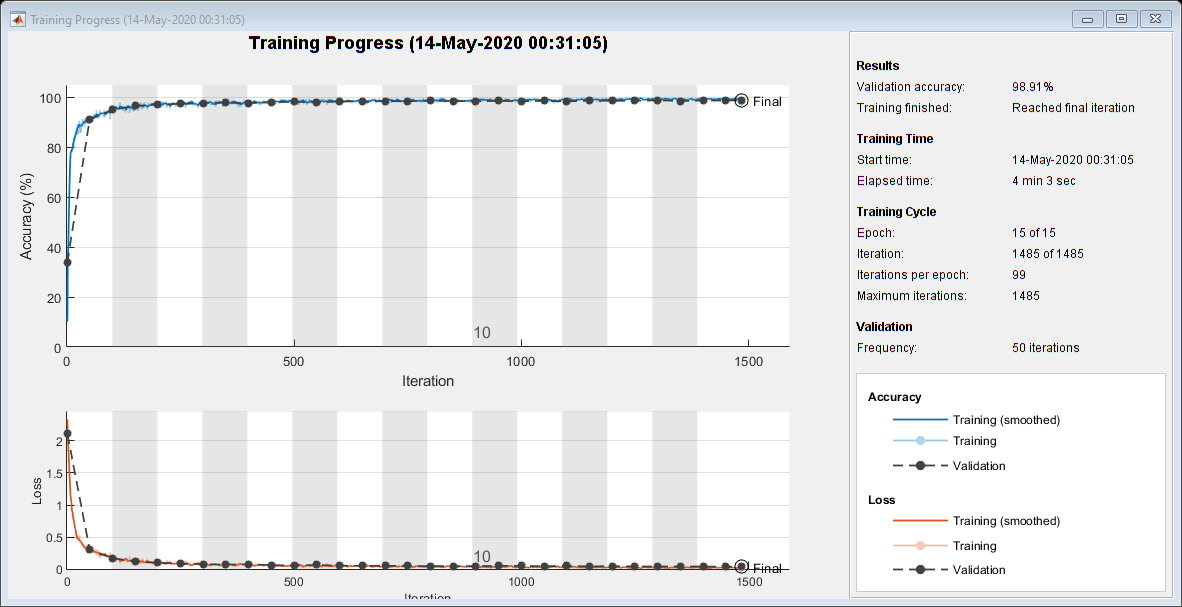
\includegraphics[width=\maxwidth{80.28098344204717em}]{figure_3.png}
\end{center}
\pagebreak

\label{T_F69C5DEE}
\matlabtitle{2. Confusion Matrices (10x10) of LeNet-5}

\begin{par}
\begin{flushleft}
Here we will use the test partition of the dataset to evaluate the trained network.
\end{flushleft}
\end{par}

\label{H_1196D867}
\matlabheading{2.1 Loading the Test Set of MNIST}

\begin{matlabcode}
rootFolder = 'mnistTest';
imds_test = imageDatastore(fullfile(rootFolder, categories), ...
    'LabelSource', 'foldernames');
clear rootFolder

disp(countEachLabel(imds_test));
\end{matlabcode}
\begin{matlaboutput}
    Label    Count
    _____    _____

      0       980 
      1      1135 
      2      1032 
      3      1010 
      4       982 
      5       892 
      6       958 
      7      1028 
      8       974 
      9      1009 
\end{matlaboutput}


\label{H_1AF6D024}
\matlabheading{2.2 Classifying Test and Train Datasets}

\begin{par}
\begin{flushleft}
The 2 lines below will classify all images in the train and test datasets.
\end{flushleft}
\end{par}

\begin{matlabcode}
predicted_labels_train_1 = classify(trained_LeNet_5, imds);
predicted_labels_test_1  = classify(trained_LeNet_5, imds_test);
\end{matlabcode}
\pagebreak

\label{H_6807B946}
\matlabheading{2.3 Plotting Cofusion Matrices}

\begin{par}
\begin{flushleft}
As the final step of this section, we will plot the confusion matrices.
\end{flushleft}
\end{par}

\label{H_C59CCAFB}
\matlabheadingtwo{2.3.1 Cofusion Matrix of Training Dataset}

\begin{par}
\begin{flushleft}
The neural network is capable of classifying the training part of the dataset with a precision of 99.5\%.
\end{flushleft}
\end{par}

\begin{matlabcode}
plotconfusion(imds.Labels, predicted_labels_train_1);
\end{matlabcode}
\begin{center}
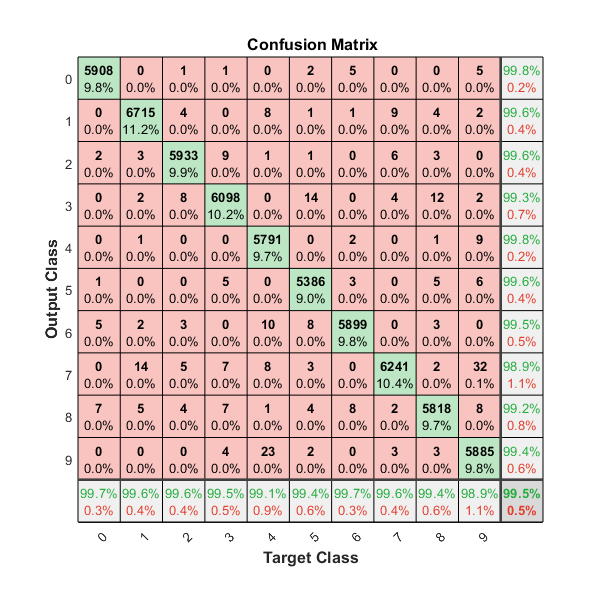
\includegraphics[width=\maxwidth{60.210737581535376em}]{figure_4.png}
\end{center}

\label{H_BD57F7D0}
\matlabheadingtwo{2.3.2 Cofusion Matrix of Test Dataset}

\begin{par}
\begin{flushleft}
The neural network has classified 98.8\% of the test dataset correctly.
\end{flushleft}
\end{par}

\begin{matlabcode}
plotconfusion(imds_test.Labels, predicted_labels_test_1);
\end{matlabcode}
\begin{center}
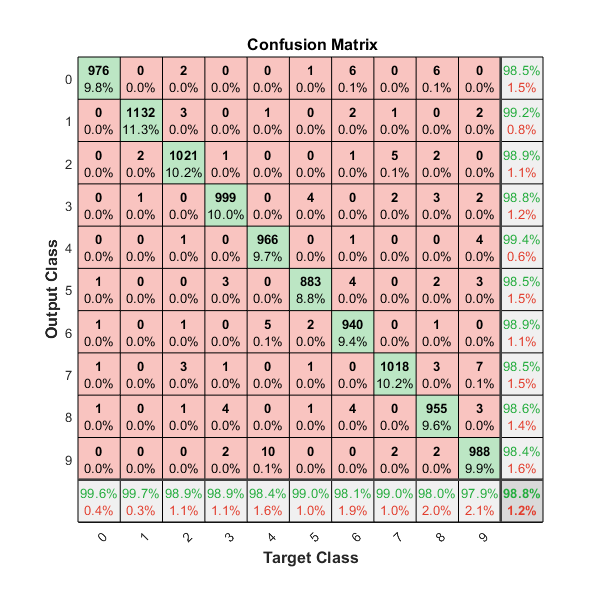
\includegraphics[width=\maxwidth{60.210737581535376em}]{figure_5.png}
\end{center}
\pagebreak

\label{T_DC6116AE}
\matlabtitle{3. Modified LeNet-5 Training}

\begin{par}
\begin{flushleft}
In this part we will remove C5 and F6 layers and retrain the network to see how it might affect the classification performance.
\end{flushleft}
\end{par}

\label{H_917F3471}
\matlabheading{1.1 Defining Modified LeNet-5 Architecture}

\begin{par}
\begin{flushleft}
The code below has defined the LeNet-5 with C5 and F6 layers removed.
\end{flushleft}
\end{par}

\begin{matlabcode}
LeNet_5_modified = [
    imageInputLayer([28 28], 'Name', 'data')
    
    convolution2dLayer([5 5], 6, 'Name', 'C1', 'Stride', [1 1], 'padding', 'same')
    tanhLayer('Name','tanh1')
    
    averagePooling2dLayer([2 2], 'Name', 'S2', 'Stride', [2 2])
    
    convolution2dLayer([5 5], 16, 'Name', 'C3', 'Stride', [1 1])
    tanhLayer('Name','tanh3')
    
    averagePooling2dLayer([2 2], 'Name', 'S4', 'Stride', [2 2])
    
    fullyConnectedLayer(10, 'Name', 'output')
    softmaxLayer('Name','softmax')
    
    classificationLayer('Name','classification')
    ];

disp(LeNet_5_modified);
\end{matlabcode}
\begin{matlaboutput}
  10x1 Layer array with layers:

     1   'data'             Image Input             28x28x1 images with 'zerocenter' normalization
     2   'C1'               Convolution             6 5x5 convolutions with stride [1  1] and padding 'same'
     3   'tanh1'            Tanh                    Hyperbolic tangent
     4   'S2'               Average Pooling         2x2 average pooling with stride [2  2] and padding [0  0  0  0]
     5   'C3'               Convolution             16 5x5 convolutions with stride [1  1] and padding [0  0  0  0]
     6   'tanh3'            Tanh                    Hyperbolic tangent
     7   'S4'               Average Pooling         2x2 average pooling with stride [2  2] and padding [0  0  0  0]
     8   'output'           Fully Connected         10 fully connected layer
     9   'softmax'          Softmax                 softmax
    10   'classification'   Classification Output   crossentropyex
\end{matlaboutput}


\begin{par}
\begin{flushleft}
In the figure below, we can see the whole network at a glance:
\end{flushleft}
\end{par}

\begin{matlabcode}
analyzeNetwork(LeNet_5_modified);
plot(layerGraph(LeNet_5_modified));
\end{matlabcode}
\begin{center}
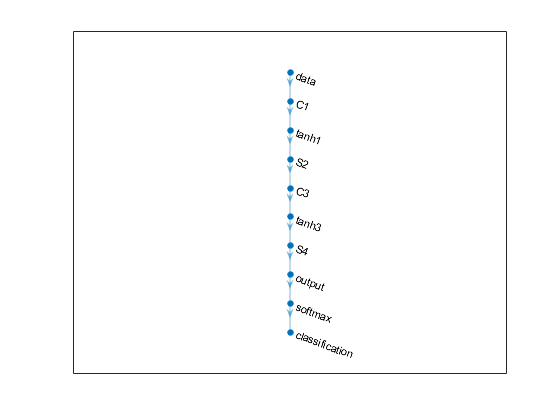
\includegraphics[width=\maxwidth{56.196688409433015em}]{figure_6.png}
\end{center}


\label{H_F206E7EE}
\matlabheading{1.2 Defining Options for Training}

\begin{par}
\begin{flushleft}
We have used 15 epoches with mini-batch size of 512, the same as the previous question.
\end{flushleft}
\end{par}

\begin{matlabcode}
opts = trainingOptions('adam', ...
    'ExecutionEnvironment','auto', ...
    'MaxEpochs', 15, ...
    'MiniBatchSize', 512, ...
    'Shuffle', 'every-epoch', ...
    'Plots', 'training-progress', ...
    'Verbose', true, ...
    'ValidationData', imdsValidation);
\end{matlabcode}


\label{H_86B9D4D5}
\matlabheading{1.4 Learning Curves and Training Process}

\begin{par}
\begin{flushleft}
We trained the network on single GPU system. The results are printed in a table every 50 iterations. Besides, the learning curves are plotted after the table. Finally the network reached 99.22\% on training and 98.21\% on validation subset. The training process took about 3 minutes long.
\end{flushleft}
\end{par}

\begin{matlabcode}
trained_LeNet_5_modified = trainNetwork(imdsTrain, LeNet_5_modified, opts);
\end{matlabcode}
\begin{matlaboutput}
Training on single GPU.
Initializing input data normalization.
|================================================================================================================|
|  Epoch  |  Iteration  |  Time Elapsed  |  Mini-batch  |  Validation  |  Mini-batch  |  Validation  |  Base Learning  |
|         |             |   (hh:mm:ss)   |   Accuracy   |   Accuracy   |     Loss     |     Loss     |      Rate       |
|================================================================================================================|
|       1 |           1 |       00:00:03 |        6.45% |        9.72% |       2.4225 |       2.2939 |          0.0010 |
|       1 |          50 |       00:00:08 |       86.91% |       87.17% |       0.5743 |       0.5366 |          0.0010 |
|       2 |         100 |       00:00:13 |       90.82% |       90.62% |       0.3270 |       0.3387 |          0.0010 |
|       2 |         150 |       00:00:18 |       92.19% |       92.30% |       0.2801 |       0.2680 |          0.0010 |
|       3 |         200 |       00:00:24 |       93.36% |       93.89% |       0.2134 |       0.2204 |          0.0010 |
|       3 |         250 |       00:00:29 |       93.95% |       94.52% |       0.2008 |       0.1870 |          0.0010 |
|       4 |         300 |       00:00:35 |       95.31% |       95.34% |       0.1802 |       0.1620 |          0.0010 |
|       4 |         350 |       00:00:40 |       95.90% |       95.87% |       0.1548 |       0.1447 |          0.0010 |
|       5 |         400 |       00:00:46 |       95.70% |       96.29% |       0.1488 |       0.1299 |          0.0010 |
|       5 |         450 |       00:00:51 |       96.09% |       96.57% |       0.1372 |       0.1185 |          0.0010 |
|       6 |         500 |       00:00:57 |       96.48% |       96.80% |       0.1190 |       0.1098 |          0.0010 |
|       6 |         550 |       00:01:02 |       96.68% |       96.97% |       0.0991 |       0.1021 |          0.0010 |
|       7 |         600 |       00:01:08 |       95.90% |       97.26% |       0.1047 |       0.0967 |          0.0010 |
|       7 |         650 |       00:01:13 |       97.85% |       97.46% |       0.0825 |       0.0897 |          0.0010 |
|       8 |         700 |       00:01:18 |       98.05% |       97.60% |       0.0718 |       0.0852 |          0.0010 |
|       8 |         750 |       00:01:24 |       97.85% |       97.67% |       0.0657 |       0.0817 |          0.0010 |
|       9 |         800 |       00:01:29 |       97.66% |       97.79% |       0.0798 |       0.0778 |          0.0010 |
|       9 |         850 |       00:01:34 |       97.66% |       97.69% |       0.0778 |       0.0758 |          0.0010 |
|      10 |         900 |       00:01:40 |       98.05% |       97.79% |       0.0696 |       0.0745 |          0.0010 |
|      10 |         950 |       00:01:45 |       98.44% |       97.88% |       0.0656 |       0.0723 |          0.0010 |
|      11 |        1000 |       00:01:51 |       98.05% |       97.97% |       0.0584 |       0.0700 |          0.0010 |
|      11 |        1050 |       00:01:56 |       96.68% |       97.98% |       0.0829 |       0.0679 |          0.0010 |
|      12 |        1100 |       00:02:02 |       97.46% |       98.06% |       0.0772 |       0.0665 |          0.0010 |
|      12 |        1150 |       00:02:07 |       98.05% |       97.91% |       0.0593 |       0.0648 |          0.0010 |
|      13 |        1200 |       00:02:12 |       98.44% |       98.03% |       0.0543 |       0.0661 |          0.0010 |
|      13 |        1250 |       00:02:17 |       98.24% |       98.11% |       0.0684 |       0.0614 |          0.0010 |
|      14 |        1300 |       00:02:23 |       98.44% |       98.04% |       0.0478 |       0.0639 |          0.0010 |
|      14 |        1350 |       00:02:28 |       97.85% |       98.14% |       0.0743 |       0.0592 |          0.0010 |
|      15 |        1400 |       00:02:33 |       98.44% |       98.27% |       0.0538 |       0.0584 |          0.0010 |
|      15 |        1450 |       00:02:38 |       98.63% |       98.12% |       0.0435 |       0.0598 |          0.0010 |
|      15 |        1485 |       00:02:42 |       99.22% |       98.21% |       0.0443 |       0.0577 |          0.0010 |
|================================================================================================================|
\end{matlaboutput}
\begin{center}
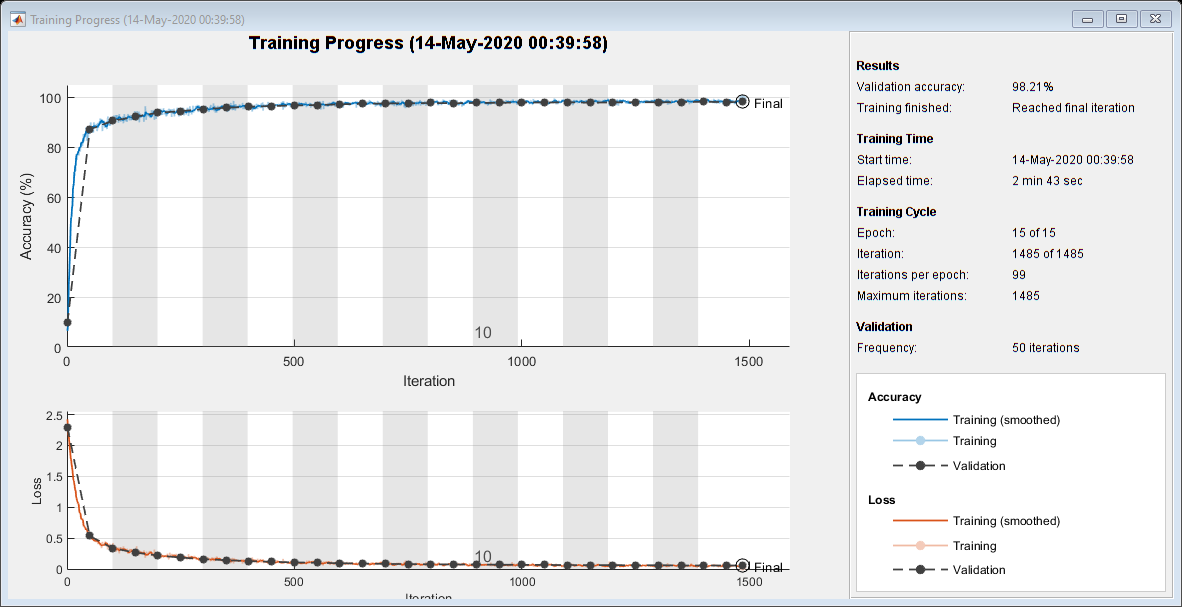
\includegraphics[width=\maxwidth{80.28098344204717em}]{figure_7.png}
\end{center}
\pagebreak

\label{T_C3AD9E71}
\matlabtitle{4. Confusion Matrices (10x10) of Modified LeNet-5}

\begin{par}
\begin{flushleft}
As the final step of this section, we will plot the confusion matrices.
\end{flushleft}
\end{par}

\label{H_884030D2}
\matlabheading{4.2 Classifying Test and Train Datasets}

\begin{par}
\begin{flushleft}
The 2 lines below will classify all images in the train and test datasets.
\end{flushleft}
\end{par}

\begin{matlabcode}
predicted_labels_train_2 = classify(trained_LeNet_5_modified, imds);
predicted_labels_test_2  = classify(trained_LeNet_5_modified, imds_test);
\end{matlabcode}
\pagebreak

\label{H_9CA06B14}
\matlabheading{4.3 Plotting Cofusion Matrices}

\begin{par}
\begin{flushleft}
As the final step of this section, we plot the confusion matrix.
\end{flushleft}
\end{par}

\label{H_B0BB8B56}
\matlabheadingtwo{4.3.1 Cofusion Matrix of Training Dataset}

\begin{par}
\begin{flushleft}
The neural network is capable of classifying the training part of the dataset with a precision of 98.5\%. Removing the two layers has degraded performance on training dataset for 1 percent.
\end{flushleft}
\end{par}

\begin{matlabcode}
plotconfusion(imds.Labels, predicted_labels_train_2);
\end{matlabcode}
\begin{center}
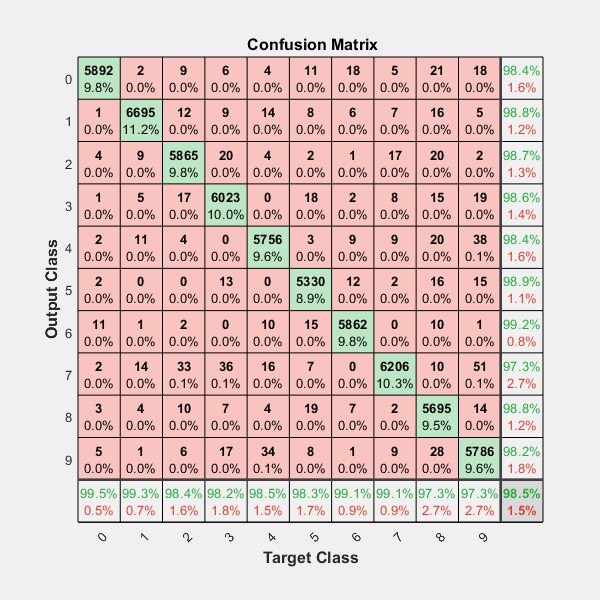
\includegraphics[width=\maxwidth{60.210737581535376em}]{figure_8.png}
\end{center}

\label{H_4D413825}
\matlabheadingtwo{4.3.2 Cofusion Matrix of Test Dataset}

\begin{par}
\begin{flushleft}
The neural network has classified 98.5\% of the test dataset correctly which is 0.3 percent degradation in performance in comparison to the original LeNet-5 that was trained in the previous question.
\end{flushleft}
\end{par}

\begin{matlabcode}
plotconfusion(imds_test.Labels, predicted_labels_test_2);
\end{matlabcode}
\begin{center}
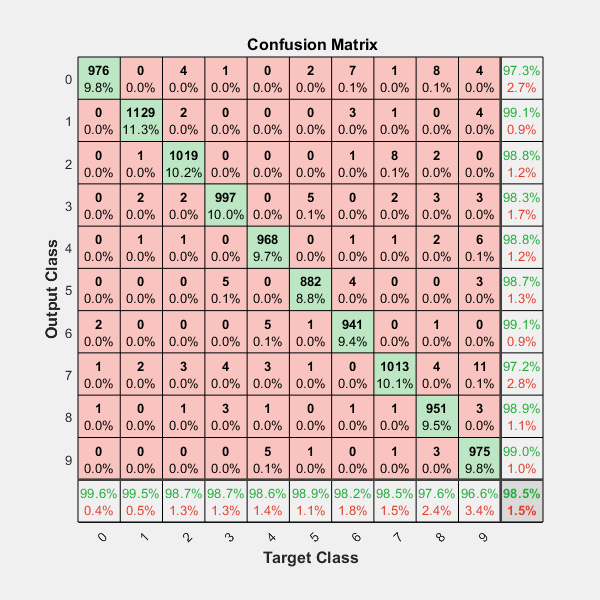
\includegraphics[width=\maxwidth{60.210737581535376em}]{figure_9.png}
\end{center}
\pagebreak

\label{T_F8AA430C}
\matlabtitle{Appendix}

\label{H_64B544B3}
\matlabheading{A.1 Saving Workspace Variables for Future Use }

\begin{matlabcode}
save('HW10_code_workspace.mat')
\end{matlabcode}


\label{H_430FCF21}
\matlabheading{A.2 Defiition of Auxiliary Functions}

\begin{matlabcode}
function downloadMNIST(mnist_train_image, mnist_train_label, mnist_test_image, mnist_test_label)

if exist('train-images-idx3-ubyte','file') ~= 2
    disp('Downloading MNIST dataset...');
    websave([mnist_train_image,'.gz'],...
        ['http://yann.lecun.com/exdb/mnist/', ...
        mnist_train_image, '.gz']);
    websave([mnist_train_label,'.gz'],...
        ['http://yann.lecun.com/exdb/mnist/', ...
        mnist_train_label, '.gz']);
    websave([mnist_test_image,'.gz'],...    
        ['http://yann.lecun.com/exdb/mnist/', ...
        mnist_test_image, '.gz']);
    websave([mnist_test_label,'.gz'],...
        ['http://yann.lecun.com/exdb/mnist/', ...
        mnist_test_label, '.gz']);
    disp('MNIST dataset downloded.');
    
    disp('Unzipping started...');
    gunzip([mnist_train_image, '.gz'])
    gunzip([mnist_train_label, '.gz'])
    gunzip([mnist_test_image, '.gz'])
    gunzip([mnist_test_label, '.gz'])
    delete([mnist_train_image, '.gz'])
    delete([mnist_train_label, '.gz'])
    delete([mnist_test_image, '.gz'])
    delete([mnist_test_label, '.gz'])
    disp('Unzipping completed.');
else
    disp('MNIST dataset already downloaded.')
end

end

function [imgs, labels] = readMNIST(imgFile, labelFile, num_of_digits_to_read)

fileID = fopen(imgFile, 'r', 'b');
header = fread(fileID, 1, 'int32');

if header ~= 2051
    error('Invalid image file header');
end

count = fread(fileID, 1, 'int32');

if count < num_of_digits_to_read
    error('Trying to read too many digits');
end

rows_num = fread(fileID, 1, 'int32');
cols_num = fread(fileID, 1, 'int32');

imgs = zeros([rows_num cols_num num_of_digits_to_read]);

for i = 1:num_of_digits_to_read
    for row = 1:rows_num
        imgs(row, :, i) = fread(fileID, cols_num, 'uint8');
    end
end

fclose(fileID);

fileID = fopen(labelFile, 'r', 'b');
header = fread(fileID, 1, 'int32');

if header ~= 2049
    error('Invalid label file header');
end

count = fread(fileID, 1, 'int32');

if count < num_of_digits_to_read
    error('Trying to read too many digits');
end

labels = fread(fileID, num_of_digits_to_read, 'uint8');

fclose(fileID);

imgs = double(imgs)./255.0;

end

function iMontage(images)
montage(reshape(images, [28 28 size(images, 2)]), 'BackgroundColor', 'white', 'BorderSize', [2 2]);
end

function display_original_images_vs_reconstructed(original_images, reconstructed_images)
figure('Position', [100, 100, 1000, 500]);
subplot(1, 2, 1);
iMontage(original_images);
title('Original Images');
hold on;
subplot(1, 2, 2);
iMontage(reconstructed_images);
title('Reconstructed Images')
hold off
end

function categorized_label = iCategorical(on_hot_encoded_label)
[ind, ~]= vec2ind(on_hot_encoded_label);
categorized_label = categorical(ind', 1:10, {'0' '1' '2' '3' '4' '5' '6' '7' '8' '9'});
end




function saveMNISTasFolderOfImages(outputPath, train_images, train_labels, test_images, test_labels)

if(~isempty(outputPath))
    assert(exist(outputPath,'dir') == 7);
end

% Set names for directories
trainDirectoryName = 'mnistTrain';
testDirectoryName = 'mnistTest';

% Create directories for the output
mkdir(fullfile(outputPath, trainDirectoryName));
mkdir(fullfile(outputPath, testDirectoryName));

labelNames = {'0','1','2','3','4','5','6','7','8','9'};
iMakeTheseDirectories(fullfile(outputPath, trainDirectoryName), labelNames);
iMakeTheseDirectories(fullfile(outputPath, testDirectoryName), labelNames);


iLoadBatchAndWriteAsImagesToLabelFolders(train_images, fullfile(outputPath, trainDirectoryName), labelNames, train_labels);

iLoadBatchAndWriteAsImagesToLabelFolders(test_images, fullfile(outputPath, testDirectoryName), labelNames, test_labels);

end

function iLoadBatchAndWriteAsImagesToLabelFolders(data, fullOutputDirectoryPath, labelNames, labels)
for i = 1:size(data,3)
    imwrite(data(:,:,i), fullfile(fullOutputDirectoryPath, labelNames{labels(i)+1}, ['image' num2str(i) '.png']));
end
end

function iMakeTheseDirectories(outputPath, directoryNames)
for i = 1:numel(directoryNames)
    mkdir(fullfile(outputPath, directoryNames{i}));
end
end


function h = subplottight(n,m,i)
[c,r] = ind2sub([m n], i);
ax = subplot('Position', [(c-1)/m, 1-(r)/n, 1/m, 1/n]);
if(nargout > 0)
    h = ax;
end
end
\end{matlabcode}

\end{document}
